
\chapter{Opis projektnog zadatka}
		
		{Cilj ovog projektnog zadatka je napraviti web aplikaciju koja polaznicima treninga omogućuje rezervaciju odgovarajućeg termina treninga i postavljanje osobnih ciljeva koje žele ostvariti u nadolazećem mjesecu, a terenima daje mogućnost planiranja i treninga ovisno prema ciljevima korisnika i daje im mogućnosti postavljanja ograničenja za treninge.\\}
		
		
		{Potreba za razvojem ovakve aplikacije iz klijentske perspektive javlja se zbog velikog broja obaveza i nemogućnosti praćenja fiksnog rasporeda treninga. Kako korisnici ne mogu pohađati svaki trening, javlja se nezadovoljstvo iz dva razloga:}
		
		\begin{packed_item}
		    \item {nemogućnost pohađanja usluge koju su platili}
		    \item {usporen napredak zbog neredovitog treniranja}
		\end{packed_item}
		
		{Kako treneri ne bi gubili klijente, nudimo im mogućnost pohađanja termina u vrijeme kada klijentima odgovara.\\}
		
		
		{U aplikaciji, postoje dvije role koje korisnik može odabrati:}
		
		\begin{packed_item}
		    \item {klijent (u daljnjem tekstu vježbač)}
		    \item {trener}
		\end{packed_item}
		
		{Pri pokretanju aplikacije, ukoliko korisnik već nema postojeći račun, mora izvršiti registraciju. Pri registraciji, korisnik mora unijeti određene podatke:}
		
		\begin{packed_item}
		    \item {ime}
		    \item {prezime}
		    \item {datum rođenja}
		    \item {email adresa}
		    \item {korisničko ime}
		    \item {kontakt broj}
		    \item {lozinka}
		    \item {tip korisnika (vježbač ili trener)}
		    \begin{packed_item}
		        \item {ako je tip vježbač, potrebno je unijeti i cilj}
		    \end{packed_item}
		\end{packed_item}
		
		{
		Lozinka koju korisnik unese mora imati 8 – 20 znakova.\\}
		
		{Pri registraciji, vježbač odabire vlastiti cilj na temelju kojeg mu trener određuje treninge. Postoje tri različita cilja koja korisnik može odabrati:}
		
		\begin{packed_item}
            \item {povećanje mišićne mase}
            \item {izdržljivost}
            \item {gubitak težine }
        \end{packed_item}
        
        % {Treninzi za svaki cilj su različiti i zbog toga postoje četiri različite vrste treninga:}
        
        % \begin{packed_item}
        %     \item {„bodyweight“ trening}
        %     \item {trening s utezima}
        %     \item {trening snage}
        %     \item {„cardio“ trening}
        % \end{packed_item}
		
		% {Tako, ukoliko vježbač želi povećati snagu, treninzi izdržljivosti usporili bi ga na putu ka tom cilju, pa mu ih trener neće dodijeliti.\\}
		
		{Kada se vježbač registrira, dobiva potvrdni mail za registraciju koji ga odvodi na stranicu za prijavu. Po dodjeli treninga vježbaču se unutar aplikacije prikazuju njemu dodijeljeni treninzi (i termini istih).\\}
		
		
		{Kada netko od trenera vježbaču dodijeli fond sati koji vježbač može iskoristiti i kada vježbač dobije ponuđene treninge, vježbač dobiva obavijest na mail te može na kalendaru odabrati termine u kojima bi htio odraditi treninge. Treninzi se odrađuju u nekoliko termina svaki radni dan:}
		
		\begin{packed_item}
            \item {8:00 sati}
            \item {10:00 sati}
            \item {12:00 sati}
            \item {14:00 sati}
            \item {16:00 sati}
            \item {18:00 sati}
            \item {20:00 sati}

        \end{packed_item}
        
        {Ako vježbač ipak ne može pohađati trening za koji se prijavio, moguće je poništiti rezervaciju bez gubitka fonda sati.\\}
        
        {Vježbač može nakon nekog vremena, ili na samom početku, izgubiti volju ili motivaciju za određenom vrstom treninga i zbog toga mu moramo omogućiti određenu fleksibilnost. Zadnji tjedan u mjesecu, vježbaču ćemo omogućiti promjenu cilja.}
        
        {Kada vježbač rezervira termin, njegov fond sati se umanjuje za duljinu trajanja treninga koja je u našem slučaju 2h. S druge strane, otkazivanjem rezervacije, njegov fond sati se uvećava za duljinu treninga, tako da rezervacija te otkaz iste nemaju utjecaj na korisnikov fond sati.\\}
		
		{Ako vježbač odluči ne doći na trening, ukoliko nije poništio rezervaciju, rezervirani trening se računa kao odrađeni, iako ga vježbač nije pohađao. Time vježbači gube mogućnost naknadnog odrađivanja rezerviranog treninga.\\}
		
		
		{Radi ograničenog broja opreme, treneri moraju definirati i maksimalan broj polaznika za određenu vrstu treninga. Kada su sva slobodna mjesta za određeni trening popunjena, termin nestaje iz aplikacije i korisnici ga više ne mogu vidjeti.\\}
		
		{Treneri trebaju napraviti raspored treninga prema određenim ciljevima vježbača kako bi vježbači mogli što prije ispuniti svoje ciljeve i biti zadovoljni pruženom uslugom.\\}
		
		{Kao primjer, uzmimo vježbača koji želi povećati izdržljivost. Trener u skladu s ciljem vježbača treba uzeti u obzir fond sati koji bi odgovarali za postizanje navedenog cilja te na temelju oba faktora odrediti koliko različitih vrsta treninga vježbač treba odraditi.\\}
		
		
		{Iako više treninga može biti "tipa" trening snage (što će često biti vidljivo u nazivu treninga), to ne znači da svi treninzi istog ili sličnog naziva nužno sadrže iste vježbe. Treneru je dano na vlastitu prosudbu da pri izradi treninga definira koje vježbe isti obuhvaća. \\}


        {Za vježbače postoji ograničenje na broj mogućih rezervacija termina treninga tjedno. Ograničenje je skalirano prema fondu sati koje je vježbaču dodijeli trener, tj. vježbači sa velikim fondom sati imaju mogućnost većeg broja rezervacija tjedno u odnosu na manji fond sati. \\}
		
        
        {Ako vježbač pokuša prekršiti ograničenje broja mogućih rezervacija, aplikacija ga o tome obavijesti porukom i ne dopušta mu izvršavanje rezervacije koja krši zadano pravilo.\\}
        
        {Uz unaprijed definirano pravilo koje provjerava aplikacija, treneri mogu pri izradi treninga napisati vlastita pravila (u sklopu opisa treninga).\\}
        
        {Administrator je uloga koja ima mogućnosti upravljanja korisničkim računima (brisanje računa) te verifikaciju trenera.\\
        Pri registraciji, korisnik odabire ulogu trenera ili vježbača. Kako se bilo tko ne bi mogao neovlašteno registrirati kao trener, administrator mora potvrditi (verificirati) registraciju trenera.\\
        Nema mogućnost mijenjati raspored ili program koji su treneri definirali.\\}

        
        {Aplikacija je dostupna na "\href{https://group-fitness-planer-q3fc.onrender.com}{Group Fitness Planner.}"}
		\eject

        \section{Pregled konkurentskih rješenja i analiza tržišta\\}

        {Istražujući na internetu, naišli smo na nekolicinu aplikacija sa sličnim namjenama kao što je i naša. Kako se teži digitalizaciji i navika ljudi je glavninu informacija o onome što ih zanima pronaći na internetu, tako i razna poduzeća teže imati kompletnu i interaktivnu internetsku uslugu preko koje se reklamiraju, organiziraju, a ponekad i djeluju raznim on-line sadržajima. \\ \\ }
        {Primjerice, servis Exercise (\href{https://www.exercise.com}{https://www.exercise.com/}) nudi jedinstvenu platformu za upravljanje fitness ustanovom, od mogućnosti registracije polaznika i pretplatnika na usluge, zaposlenika i voditelja, do registracije lokacija na kojima se odvijaju aktivnosti, e-potpisivanja ugovora i pretplata, kreiranja treninga, TV-treninga i biblioteke treninga i vježbi, statistike dolazaka na treninge, izvješća o napredovanju, online live prijenosa, izazova…}
        
              \begin{figure}[H]
                      
\includegraphics[scale=0.5]{./Slike/trainer_workouts.png}
                      \centering
                      \caption{Exercise}
                      \label{fig:promjene}
                \end{figure}

                \begin{figure}[H]
                      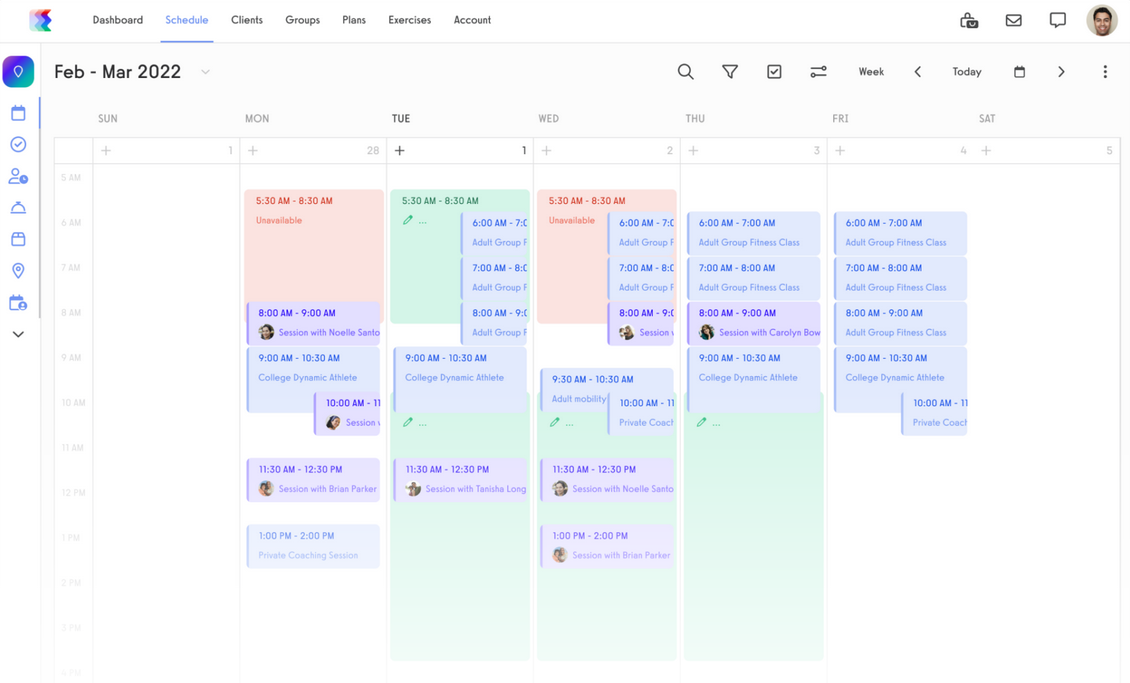
\includegraphics[scale=0.5]{./Slike/trainer_schedule.png}
                      \centering
                      \caption{Exercise}
                      \label{fig:promjene}
                \end{figure}

                \begin{figure}[H]
                      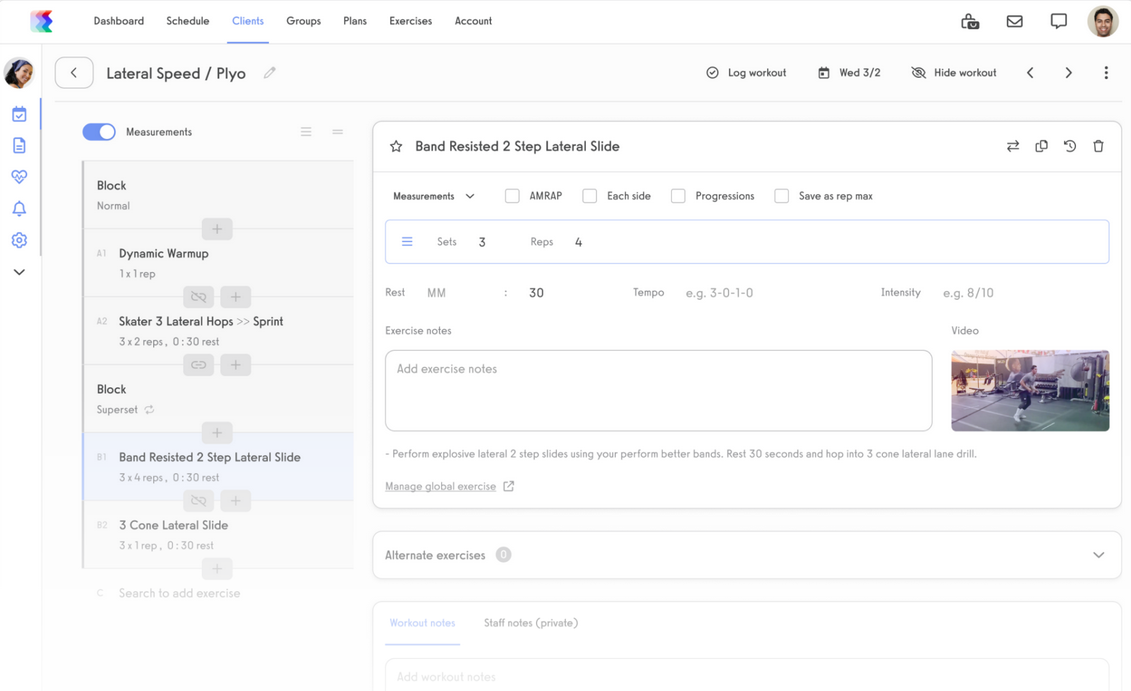
\includegraphics[scale=0.5]{./Slike/trainer_client.png}
                      \centering
                      \caption{Exercise}
                      \label{fig:promjene}
                \end{figure}

                 \begin{figure}[H]
                      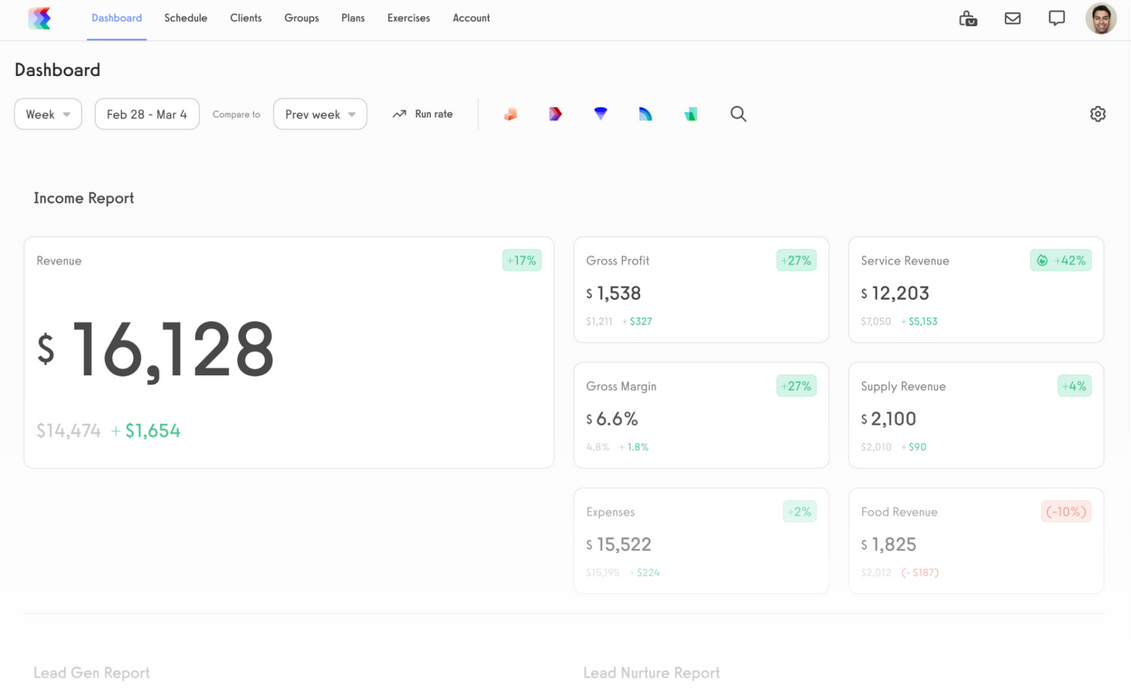
\includegraphics[scale=0.5]{./Slike/stats.png}
                      \centering
                      \caption{Exercise}
                      \label{fig:promjene}
                \end{figure}
        {Exercise obuhvaća puno veći spektar usluga nego što obuhvaća naša „Group fitness planner“ aplikacija, pa je samim time naša aplikacija namijenjena užem krugu klijenata. Ciljani klijenti su manji fitness centri sa jednim prostorom za vježbanje, koji pomoću dobre organizacije i individualiziranog pristupa treninzima žele steći povjerenje kod svojih korisnika i imati maksimalnu učinkovitost u pogledu prilagođavanja vrste i termina treninga po želji i mogućnostima svojih korisnika. Aplikacija je jednostavna i intuitivna za korištenje, te sa samo nekoliko funkcionalnosti ispunjava svrhu opisanu opisom projektnog zadatka. \\ \\}
                \begin{figure}[H]
                      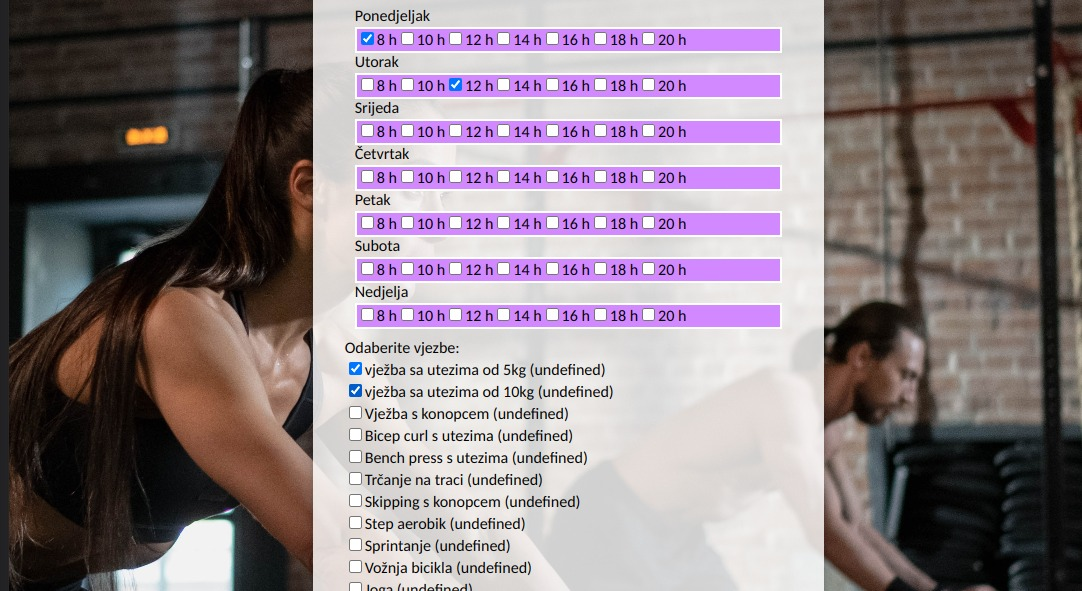
\includegraphics[scale=0.4]{./Slike/front.png}
                      \centering
                      \caption{Group fitness planner}
                      \label{fig:promjene}
                \end{figure}

        {Osim opisanog servisa Excercise, na tržištu su dostupni i sljedeći servisi: Mindbody \href{https://www.mindbodyonline.com/business/fitness-software}{(https://www.mindbodyonline.com/business/fitness-software)} aplikacija koja ima mnoge verzije, a svaka je prilagođena tipu poduzeća (za frizere, za fitness centre, za sportske klubove, za studije ljepote…) i ovisno o verziji sadržava funkcionalnosti potrebne za upravljanje tim poduzećem što intenzivno širi područja primjene aplikacije i skupinu ciljanih klijenata, Zenplanner \href{https://zenplanner.com/}{(https://zenplanner.com/)}... \\ }

        {Da bismo dobili uvid u stvarni interes potencijalnih kupaca našeg proizvoda odlučili smo kontaktirati lokalni sportski klub i postaviti trenerima i polaznicima u klubu Google forms upitnik \href{https://docs.google.com/forms/d/e/1FAIpQLSenHBNtxCLnlzAUZP_xeXSPl-oNTVsIt4iL1JYWlX9hdUSjcg/viewform?usp=sf_link}{(https://docs.google.com/forms)} .\\ }

        {Rezultati upitnika nalažu da su mišljenja oko aplikacije podijeljena. Dok su vježbači oduševljeno prihvatili osmišljeni sustav, treneri su rezerviraniji prema njemu i vide moguće nedostatke. \\Vježbači se apsolutno slažu sa idejom o plaćanju treninga po terminima (umjesto mjesečno, unaprijed), te sa mogućnošću dolaska na različite tipove treninga, koji se poklapaju sa njihovim ciljevima. \\Zanimljivo je istaknuti kako vježbači smatraju da je određivanje fitness ciljeva na mjesečnoj bazi prečesto, te se sugerira timu da u budućem radu obrati pozornost na taj podatak. }
                \begin{figure}[H]
                      
\includegraphics[scale=0.8]{./Slike/vježbači.png}
                      \centering
                      \caption{Rezultati ankete}
                      \label{fig:promjene}
                \end{figure}
                \begin{figure}[H]
                      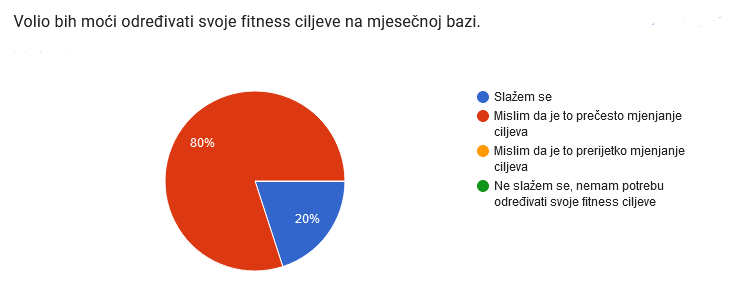
\includegraphics[scale=0.7]{./Slike/mjenjanjeciljeva.png}
                      \centering
                      \caption{Rezultati ankete}
                      \label{fig:promjene}
                \end{figure}
        {Također, vježbači su sugerirali da bi u ovakvoj aplikaciji voljeli vidjeti status svog napretka. Budućnost razvoja ovakve aplikacije mogla bi se usmjeriti na to, da uz postojeće funkcionalnosti, implementira i podatke o dolascima i redovitosti te napraviti stranicu sa statistikama konzistentnosti i napretka u postizanju željenih ciljeva. Također, voljeli bi imati „objašnjenja“ i neke osnovne edukativne materijale na stranici o tome koji su treninzi potrebni za koje ciljeve, koliko često se treba trenirati, koliko intenzivno… Iako smo mi na to vodili računa u implementaciji, korisnik iz korisničkog sučelja nema takav dojam, a aplikacija bi trebala biti jednostavna i intuitivna, te „voditi te“ kroz fitness iskustvo. \\}

        {Treneri su skeptični prema ovakvoj aplikaciji jer smatraju da bi kvaliteta njihovog rada bila značajno umanjena, ponajviše time što ne bi imali stalne grupe polaznika na koje mogu računati, i koje već poznaju, pa time i pomažu i prilagođavaju određene zadatke. Smatraju kako bi pod izlikom „danas mi ne odgovara dani termin, pa ću odraditi neki drugi trening“ klijenti otežavali i usporavali dostizanje određenih ciljeva. Također, smatraju da u klasičnim grupama s vremenom mogu zadavati sve teže i dinamičnije treninge, kako ljudi napreduju. Na ovakvim treninzima, uvijek bi bilo ljudi sa svim stupnjevima vještine, od početnika do iskusnih, te da bi bilo teško osmišljavati treninge takvim grupama. \\}

        {Pri razvoju svakako treba poštovati mišljenja stručnjaka i naći rješenje koje će djelomično zadovoljavati obje strane. Treneri predlažu da se treninzi, uz obzir na odabir ciljeva, dijele i prema stupnju fizičke spreme. Da stari i novi polaznici imaju svoje zasebne termine, i da sustav prepoznaje da je neki vježbač prvih mjesec-dva po registraciji „početnik“, osim ako vježbač zbog svoje prethodne sportske podloge ne zatraži drugačije. \\}
            
		\eject

        